\documentclass[a4paper,14pt, unknownkeysallowed]{extreport}

\usepackage{cmap} % Улучшенный поиск русских слов в полученном pdf-файле
\usepackage[T2A]{fontenc} % Поддержка русских букв
\usepackage[utf8]{inputenc} % Кодировка utf8
\usepackage[english,russian]{babel} % Языки: русский, английский
\usepackage{enumitem}


\usepackage{threeparttable}

\usepackage[14pt]{extsizes}

\usepackage{caption}
\captionsetup{labelsep=endash}
\captionsetup[figure]{name={Рисунок}}

% \usepackage{ctable}
% \captionsetup[table]{justification=raggedleft,singlelinecheck=off}

\usepackage{amsmath}

\usepackage{geometry}
\geometry{left=30mm}
\geometry{right=15mm}
\geometry{top=20mm}
\geometry{bottom=20mm}

\usepackage{titlesec}
\titleformat{\section}
	{\normalsize\bfseries}
	{\thesection}
	{1em}{}
\titlespacing*{\chapter}{0pt}{-30pt}{8pt}
\titlespacing*{\section}{\parindent}{*4}{*4}
\titlespacing*{\subsection}{\parindent}{*4}{*4}

\usepackage{setspace}
\onehalfspacing % Полуторный интервал

\frenchspacing
\usepackage{indentfirst} % Красная строка
\setlength{\parindent}{1.25cm}

\usepackage{titlesec}
\titleformat{\chapter}{\LARGE\bfseries}{\thechapter}{20pt}{\LARGE\bfseries}
\titleformat{\section}{\Large\bfseries}{\thesection}{20pt}{\Large\bfseries}

\usepackage{multirow}
\usepackage{listings}
\usepackage{xcolor}
\usepackage{longtable}

% Для листинга кода:
\lstset{ %
language=caml,                 % выбор языка для подсветки (здесь это С)
basicstyle=\small\sffamily, % размер и начертание шрифта для подсветки кода
numbers=left,               % где поставить нумерацию строк (слева\справа)
stepnumber=1,                   % размер шага между двумя номерами строк
numbersep=5pt,                % как далеко отстоят номера строк от подсвечиваемого кода
showspaces=false,            % показывать или нет пробелы специальными отступами
showstringspaces=false,      % показывать или нет пробелы в строках
showtabs=false,             % показывать или нет табуляцию в строках
frame=single,              % рисовать рамку вокруг кода
tabsize=2,                 % размер табуляции по умолчанию равен 2 пробелам
captionpos=t,              % позиция заголовка вверху [t] или внизу [b] 
breaklines=true,           % автоматически переносить строки (да\нет)
breakatwhitespace=false, % переносить строки только если есть пробел
escapeinside={\#*}{*)}   % если нужно добавить комментарии в коде
}



% plot
\usepackage{graphicx}
\usepackage{pgfplots}
\usepackage{filecontents}
\usetikzlibrary{datavisualization}
\usetikzlibrary{datavisualization.formats.functions}

\graphicspath{ {img/} }


\usepackage{subcaption}

\captionsetup{labelsep=endash}
\captionsetup[figure]{name={Рисунок}}



\usepackage[justification=centering]{caption} % Настройка подписей float объектов

\usepackage[unicode,pdftex]{hyperref} % Ссылки в pdf
\hypersetup{hidelinks}

\usepackage{csvsimple}

\newcommand{\code}[1]{\texttt{#1}}

\newcommand{\specialcell}[2][c]{%
  \begin{tabular}[#1]{@{}c@{}}#2\end{tabular}}

\begin{document}
	
\begin{titlepage}
	\newgeometry{pdftex, left=2cm, right=2cm, top=2.5cm, bottom=2.5cm}
	\fontsize{12pt}{12pt}\selectfont
	\noindent \begin{minipage}{0.15\textwidth}
		
\includegraphics[width=\linewidth]{img/main_logo.jpg}
	\end{minipage}
	\noindent\begin{minipage}{0.9\textwidth}\centering
		\textbf{Министерство науки и высшего образования Российской Федерации}\\
		\textbf{Федеральное государственное бюджетное образовательное учреждение высшего образования}\\
		\textbf{«Московский государственный технический университет имени \newline Н. Э. Баумана}\\
		\textbf{(национальный исследовательский университет)»}\\
		\textbf{(МГТУ им. Н. Э.~Баумана)}
	\end{minipage}
	
	\noindent\rule{18cm}{3pt}
	\newline\newline
	\noindent ФАКУЛЬТЕТ $\underline{\text{«Информатика и системы управления»~~~~~~~~~~~~~~~~~~~~~~~~~~~~~~~~~~~~~~~~~~~~~~~~~~~~~~~}}$ \newline\newline
	\noindent КАФЕДРА $\underline{\text{«Программное обеспечение ЭВМ и информационные технологии»~~~~~~~~~~~~~~~~~~~~~~~}}$\newline\newline\newline\newline\newline\newline\newline
	
	
	\begin{center}
		\noindent\begin{minipage}{1.3\textwidth}\centering
		\Large\textbf{   ~~~ Лабораторная работа №7}\newline
		\textbf{по дисциплине "Анализ Алгоритмов"}\newline\newline\newline
		\end{minipage}
	\end{center}
	
	\noindent\textbf{Тема} 			$\underline{\text{Муравьиный алгоритм}}$\newline\newline
	\noindent\textbf{Студент} 		$\underline{\text{Светличная А.А.}}$\newline\newline
	\noindent\textbf{Группа} 		$\underline{\text{ИУ7-53Б}}$\newline\newline
	\noindent\textbf{Преподаватель} $\underline{\text{Волкова Л. Л., Строганов Ю.В.}}$\newline
	
	\begin{center}
		\vfill
		Москва~---~\the\year
		~г.
	\end{center}
	\restoregeometry
\end{titlepage}
	
	\setcounter{page}{2}
	\tableofcontents
	
\newpage
\chapter*{Введение}
	
\addcontentsline{toc}{chapter}{Введение}

Муравьиный алгоритм --- один из эффективных полиномиальных алгоритмов для нахождения приближённых решений задачи коммивояжёра, а также решения аналогичных задач поиска маршрутов на графах. Суть подхода заключается в анализе и использовании модели поведения муравьёв, ищущих пути от колонии к источнику питания, и представляет собой метаэвристическую оптимизацию.
	
\chapter{Аналитическая часть}
	
\section{Цель и задачи}

\textbf{Целью} данной лабораторной работы является изучение муравьиного алгоритма на примере задачи коммивояжера.

Для достижения поставленной цели необходимо выполнить следующие \textbf{задачи}:

\begin{enumerate}
	\item[1)] исследовать задачу коммивояжера;
	\item[2)] изучить алгоритм полного перебора и муравьиный алгоритм для решения задачи коммивояжера;
	\item[3)] провести параметризацию муравьиного алгоритма на нескольких классах данных;
	\item[4)] составить схемы используемых алгоритмов;
	\item[5)] реализовать алгоритмы полного перебора и муравьиный алгоритм;
	\item[6)] провести сравнительный анализ времени работы данных алгоритмов;
	\item[7)] описать и обосновать полученные результаты в отчете.
\end{enumerate}

\section{Задача коммивояжера}

В задаче коммивояжера рассматривается $n$ ݊городов и матрица попарно различных расстояний между ними.
Требуется найти такой порядок посещения городов, чтобы суммарное пройденное расстояние было минимальным, каждый город посещался ровно один раз.
Иногда условием задачи коммивояжера является возврат в тот город, с которого начинался маршрут.

\section{Алгоритм полного перебора}

Для решения задачи коммивояжера алгоритм полного перебора предполагает рассмотрение всех возможных путей в графе и выбор наименьшего из них. 
Смысл перебора состоит в том, что перебираются все варианты объезда городов и выбирается оптимальный, что гарантирует точное решение задачи.
Однако, при таком подходе количество возможных маршрутов очень быстро возрастает с ростом $n$ (сложность алгоритма равна $n!$).

\section{Муравьиный алгоритм}

Муравьиный алгоритм \cite{shtovba} --- метод решения задач коммивояжера на основании моделирования поведения колонии муравьев.

Каждый муравей определяет для себя маршрут, который необходимо пройти на основе феромона, который он ощущает во время прохождения, каждый муравей оставляет феромон на своем пути, чтобы остальные муравьи могли по нему ориентироваться. В результате при прохождении каждым муравьем различного маршрута наибольшее число феромона остается на оптимальном пути.


Для каждого муравья переход из города i в город j зависит от трех составляющих: памяти муравья, видимости и виртуального следа феромона.

\begin{itemize}
    \item Память муравья --- это список посещенных муравьем городов, заходить в которые еще раз нельзя.
    Используя этот список, муравей гарантированно не попадет в один и тот же город дважды. 
    Данный список возрастает при совершении маршрута и обнуляется в начале каждой итерации алгоритма.

    \item Видимость --- величина, обратная расстоянию, рассчитывающаяся по формуле \ref{d_func}.
        \begin{equation}
	   \label{d_func}
	   \eta_{ij} = 1 / D_{ij},
        \end{equation} 
        где $D_{ij}$ --- расстояние между городами $i$ и $j$. 
        Видимость --- это локальная статическая информация, выражающая эвристическое желание посетить город $j$ из города $i$, то есть чем ближе город, тем больше желание посетить его.

    \item Виртуальный след феромона на ребре $(i, j)$ представляет подтвержденное муравьиным опытом желание посетить город $j$ из города $i$. Cлед феромона является глобальной и динамичной информацией --- она изменяется после каждой итерации алгоритма, отражая приобретенный муравьями опыт.
\end{itemize}

Формула вычисления вероятности перехода в заданную точку \eqref{posib}.

\begin{equation}
	\label{posib}
	P_{kij} = \begin{cases}
		\frac{\tau_{ij}^a\eta_{ij}^b}{\sum_{q=1}^m \tau^a_{iq}\eta^b_{iq}}, \textrm{вершина не была посещена ранее муравьем k,} \\
		0, \textrm{иначе,}
	\end{cases}
\end{equation}
где $a$ --- параметр влияния длины пути, $b$ --- параметр влияния феромона, $\tau_{ij}$ --- расстояния от города $i$ до $j$, $\eta_{ij}$ --- количество феромонов на ребре $(i, j)$.

Правило обновления феромона после движения всех муравьев:
\begin{equation}
	\label{update_phero_1}
		\tau_{ij}(t+1) = (1-p)\tau_{ij}(t) + \Delta \tau_{ij}.
\end{equation}

При этом
\begin{equation}
\label{update_phero_2}
 \Delta \tau_{ij} = \sum_{k=1}^N \tau^k_{ij},
\end{equation}
где
\begin{equation}
	\label{update_phero_3}
		 \Delta\tau^k_{ij} = \begin{cases}
		Q/L_{k}, \textrm{ребро посещено k-ым муравьем,} \\
		0, \textrm{иначе.}
	\end{cases}
\end{equation}

Существует несколько оптимизаций данного алгоритма, одна из которых введение так называемых элитных муравьев \cite{kureichik}. Элитный муравей усиливает ребра наилучшего маршрута, найденного с начала работы алгоритма. Количество феромона, откладываемого на ребрах наилучшего текущего
маршрута $T^+$, принимается равным $Q/L^+$, где $L^+$ — длина маршрута $T^+$. Этот феромон побуждает муравьев к исследованию решений, содержащих несколько ребер наилучшего на данный момент маршрута $T^+$. Если в муравейнике есть $e$ элитных муравьев, то ребра маршрута $T^+$ будут получать общее усиление:

\begin{equation}
	\label{opt}
		\Delta \tau_{e} = e * Q/L^+.
\end{equation}

\section*{Вывод}
	
В этом разделе была изучена задача коммивояжера и используемые для её решения алгоритмы: полный перебор и муравьиный алгоритм с оптимизацией в виде элитных муравьев.

\chapter{Конструкторская часть}

\section*{Описание алгоритмов}
\addcontentsline{toc}{section}{Описание алгоритмов}
	
На рисунке \ref{fig:full_comb_alg}, \ref{fig:ant_alg} представлены схемы алгоритма полного перебора и муравьиного алгоритма соответсвенно.

\clearpage

\begin{figure}[h!]
	\centering
	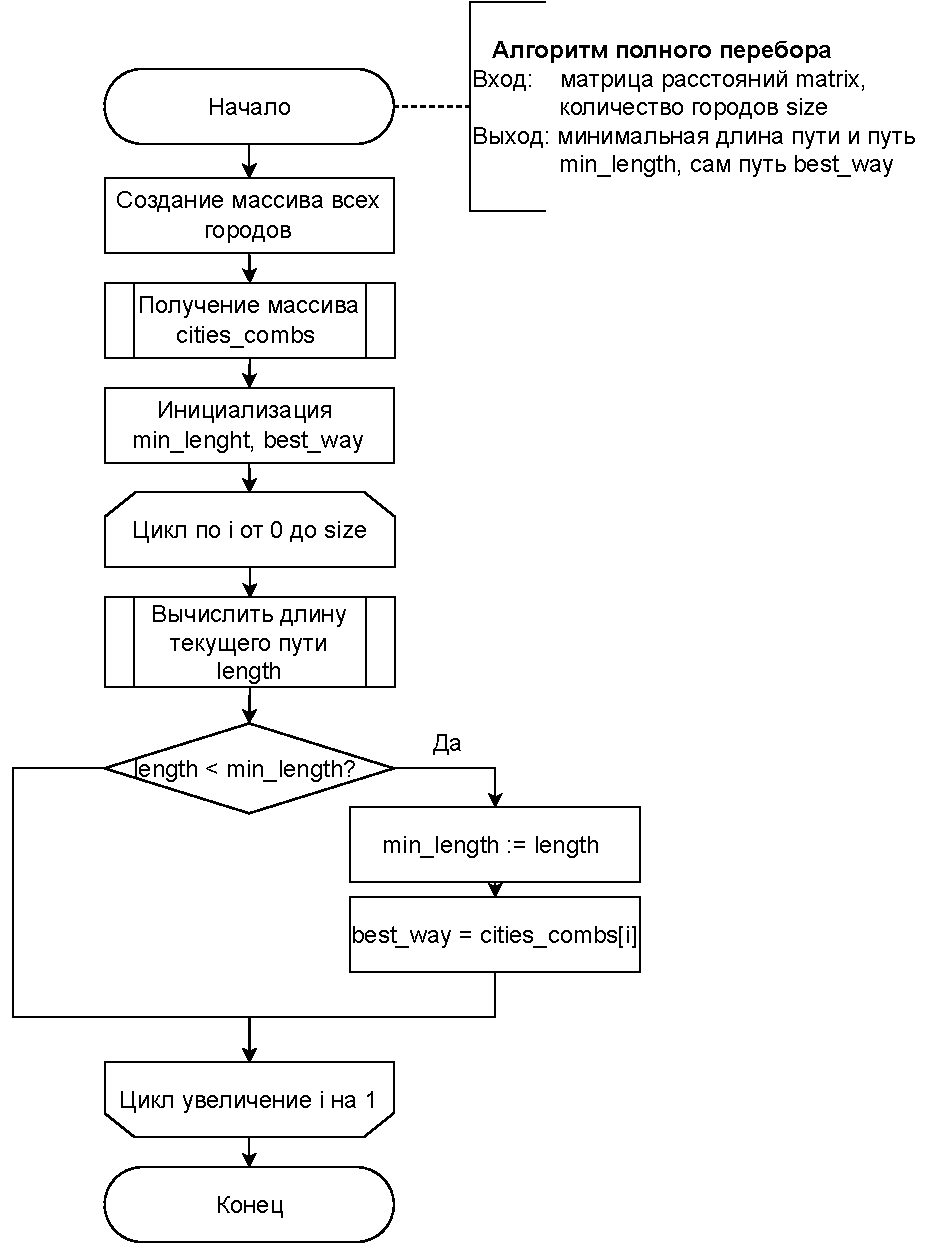
\includegraphics[width=1\linewidth]{img/full_comb_alg.pdf}
	\caption{Схема алгоритма полного перебора}
	\label{fig:full_comb_alg}
\end{figure}

\begin{figure}[h!]
	\centering
	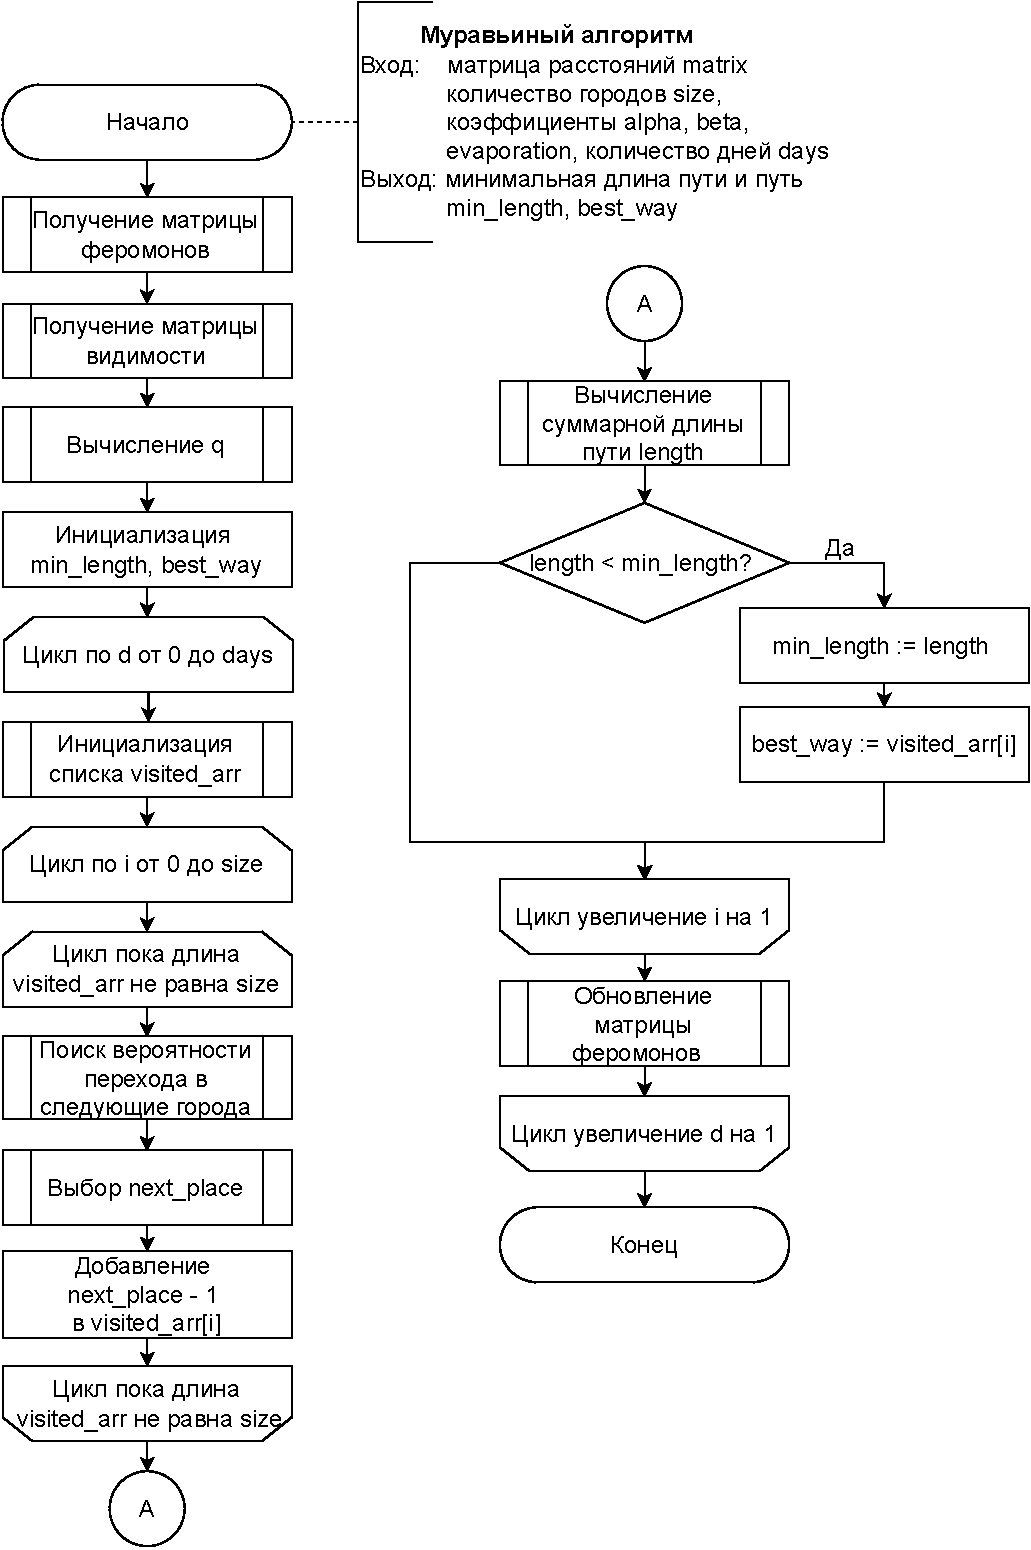
\includegraphics[width=1\linewidth]{img/ant_alg.pdf}
	\caption{Схема муравьиного алгоритма}
	\label{fig:ant_alg}
\end{figure}

\clearpage

\section*{Вывод}
	
В данном разделе на основе теоретических данных были построены схемы требуемых алгоритмов.
	
\chapter{Технологическая часть}
	
\section{Требования к программному обеспечению}

В программе должна присутствовать возможность:
	
\begin{enumerate}
	\item[1)] подавать на вход файл, содержащий матрицу смежности (расстояний), для которой можно решать задачу коммивояжера (поиск незамкнутого пути) алгоритмом полного перебора или муравьиным алгоритмом на выбор;
	\item[2)] проводить параметризацию муравьиного алгоритма для матрицы смежности, считанной из файла;
	\item[3)] замерять процессорное время выполнения алгоритмов.
\end{enumerate}
	
\section{Выбор языка программирования}
	
Для реализации программного обеспечения был выбран язык $Python$ в силу наличия модуля $numpy$, предоставляющего большое количество функций работы с массивами и матрицами.
	
\section{Выбор библиотеки и способа для замера времени}

Для замера процессорного времени выполнения реализаций агоритмов была выбрана функция $process\_time\_ns()$ из библиотеки $time$.
		
\section{Реализации алгоритмов}
	
В листингах \ref{full_comb}, \ref{ant} приведена реализация алгоритма полного перебора и муравьиного алгоритма соответственно.

\begin{lstlisting}[label=full_comb,caption=Реализация алгоритма полного перебора,language=Python]
def calc_length(matrix, size, way):
    length = 0

    for i in range(size):
        beg_city = way[i]
        end_city = way[i + 1]

        length += matrix[beg_city][end_city]

    return length

def full_combinations_alg(matrix, size):
    cities = np.arange(size)
    cities_combs = []

    for combination in it.permutations(cities):
        cities_combs.append(list(combination))

    best_way = []
    min_length = float("inf")

    for i in range(len(cities_combs)):
        length = calc_length(matrix, size - 1, cities_combs[i])

        if length < min_length:
            min_length = length
            best_way = cities_combs[i]

    return min_length, best_way
\end{lstlisting}

\clearpage

\begin{lstlisting}[label=ant,caption=Реализация муравьиного алгорима,language=Python]
def calc_q(matrix, size):
    q = 0
    count = 0

    for i in range(size):
        for j in range(size):
            if i != j:
                q += matrix[i][j]
                count += 1

    return q / count

def get_pherom_matr(size):
    pherom_matr = [[1 for i in range(size)] 
                        for j in range(size)]

    return pherom_matr

def get_visib_matr(matrix, size):
    visib_matr = [[(1.0 / matrix[i][j] if (i != j) else 0) 
                        for j in range(size)] 
                            for i in range(size)]

    return visib_matr

def get_visited_places(route, ants):
    visited_arr = [[] for i in range(ants)]

    for i in range(ants):
        visited_arr[i].append(route[i])

    return visited_arr

def update_pherom_matr(matrix, size, visited_arr, pherom_matr, q, evaporation):
    ants = size

    for i in range(size):
        for j in range(size):
            delta = 0

            for ant in range(ants):
                length = calc_length(matrix, size, visited_arr[ant])
                delta += q / length

            pherom_matr[i][j] *= (1 - evaporation)
            pherom_matr[i][j] += delta

            if pherom_matr[i][j] < MIN_PHEROMONE:
               pherom_matr[i][j] = MIN_PHEROMONE

    return pherom_matr

def choose_next_place(pk):
    size = len(pk)
    numb = 0
    i = 0

    probability = random()

    while numb < probability and i < size:
        numb += pk[i]
        i += 1

    return i

def search_probability(pherom_matr, visib_matr, visited_arr, size, ant, alpha, beta):
    pk = [0] * size

    for i in range(size):
        if i not in visited_arr[ant]:
            ant_i = visited_arr[ant][-1]

            pk[i] = pow(pherom_matr[ant_i][i], alpha) * \
                    pow(visib_matr[ant_i][i],  beta)
        else:
            pk[i] = 0

    pk_sum = sum(pk)
    
    for i in range(size):
        pk[i] /= pk_sum  

    return pk

def ant_alg(matrix, size, alpha, beta, evaporation, days):
    pherom_matr = get_pherom_matr(size)
    visib_matr  = get_visib_matr(matrix, size)

    q = calc_q(matrix, size)

    best_way = []
    min_length = float("inf")

    for j in range(days):
        visited_arr = get_visited_places(np.arange(size), size)

        for i in range(size):
            while len(visited_arr[i]) != size:
                pk = search_probability(pherom_matr, visib_matr, visited_arr, size, i, alpha, beta)  
                next_place = choose_next_place(pk)

                visited_arr[i].append(next_place - 1)

            length = calc_length(matrix, size - 1, visited_arr[i])
            
            if length < min_length:
                min_length = length
                best_way = visited_arr[i]

        pherom_matr = update_pherom_matr(matrix, size - 1, visited_arr, pherom_matr, q, evaporation)

    return min_length, best_way
\end{lstlisting}

\section{Тестирование алгоритмов}

В таблице \ref{tbl:neg_test} приведены негативные функциональные тесты, в \ref{tbl:pos_test} --- позитивные функциональные тесты для функций, реализующих алгоритм полного перебора или муравьиный алгоритм. Все тесты пройдены успешно.

\begin{table}[h]
    \captionsetup{justification=raggedright,singlelinecheck=off}
    \caption{\label{tbl:neg_test} Негативные функциональные тесты}
	\begin{center}
		\begin{tabular}{| l | l |}
			\hline
			Класс эквивалентности & Ожидаемый результат \\ \hline
   
            Номер команды не число & Введено не целое число от 0 до 4 \\\hline

            Номер команды $< 0$ или $> 4$ & Введено не целое число от 0 до 4 \\\hline

            Файл не существует & Невозможно прочитать данные файла  \\\hline

            Файл содержит не числа & Невозможно прочитать данные файла  \\\hline

            Коэффициент $\alpha$ не число & Введены неверные коэффициенты\\\hline
   
			Коэффициент $\alpha <= 0$ & Введены неверные коэффициенты\\\hline

            Коэффициент $\beta$ не число & Введены неверные коэффициенты\\\hline
   
			Коэффициент $\beta <= 0$ & Введены неверные коэффициенты\\\hline

            Коэффициент $evaporation$ не число & Введены неверные коэффициенты\\\hline
   
			Коэффициент $evaporation <= 0$ & Введены неверные коэффициенты\\\hline

            Коэффициент $days$ не число & Введены неверные коэффициенты\\\hline
   
			Коэффициент $days <= 0$ & Введены неверные коэффициенты\\\hline
   
		\end{tabular}
	\end{center}
	
\end{table}

\begin{table}[h]
    \captionsetup{justification=raggedright,singlelinecheck=off}
    \caption{\label{tbl:pos_test} Позитивные функциональные тесты}
	\begin{center}
		\begin{tabular}{|c|c|}
			\hline
			Матрица расстоян & Ожидаемый результат \\ 
			\hline

			$\begin{pmatrix}
				0 & 37 \\
				37 & 0 \\
			\end{pmatrix}$ &
			\specialcell{Минимальная сумма пути:  37 \\
            Минимальный путь:  [0, 1]} \\
			\hline
 
			$\begin{pmatrix}
                0 & 59 & 13 & 14 & 85 \\
                59 & 0 & 98 & 25 & 80 \\
                13 & 98 & 0 & 8 & 92 \\
                14 & 25 & 8 & 0 & 99 \\
                85 & 80 & 92 & 99 & 0 \\
			\end{pmatrix}$ &
		  \specialcell{Минимальная сумма пути:  126 \\
            Минимальный путь:  [0, 2, 3, 1, 4]} \\
			\hline
   
		\end{tabular}
	\end{center}
	
\end{table}

\section*{Вывод}
В данном разделе были реализованы алгоритм полного перебора, муравьиный алгоритм, а также проведено функциональное тестирование данных алгоритмов.

\chapter{Экспериментальная часть}
	
\section{Технические характеристики}
Ниже приведены технические характеристики устройства, на котором было проведено тестирование программного обеспечения:
	
\begin{enumerate}
	\item[1)] операционная система Windows-10, 64-bit;
	\item[2)] оперативная память 8 ГБ;
	\item[3)] процессор	Intel(R) Core(TM) i3-7020U CPU @ 2.30GHz, 2304 МГц, ядер 2, логических процессоров 4.
\end{enumerate}

\section{Замеры времени}

В таблице \ref{tab:time} приведены результаты замеров в миллисекундах времени работы алгоритмов полного перебора и муравьиного.

\begin{table}[h!]
    \captionsetup{justification=raggedright,singlelinecheck=off}
    \caption{Замеры времени выполнения алгоритмов на произвольных массивах разной длины}
    \label{tab:time}
	\begin{center}
        \begin{tabular}{| c | r@{.}l | r@{.}l | r@{.}l |}
        \hline
        Кол-во узлов &
        \multicolumn{2}{c|}{Полный перебор} & 
        \multicolumn{2}{c|}{Муравьиный} \\ \hline
				
        6 & 17&600 & 15&625 \\ \hline 
		
        7 & 31&250 & 62&500 \\ \hline 
				
        8 & 390&625 & 109&375 \\ \hline 
				
        9 & 3062&500 & 140&750 \\ \hline

        10 & 36625&000 & 171&875 \\ \hline
       
        \end{tabular}
    \end{center}
\end{table}

Зависимость времени работы алгоритмов полного перебора и муравьиного представлена на рисунке \ref{ris}. 
Однако в силу факториальной сложности алгоритма полного перебора удается рассмотреть только небольшую дельту размерностей матрицы, так как далее график становится нечитаемым.

\begin{center}
	\begin{figure}[h!]
	\center
	\begin{tikzpicture}
			\begin{axis} [
				legend pos = north west,
				grid = major,
                ytick={0,3100},
                minor y tick num = 10,
				xmin = 6,
				ymin = 0, 
				xmax = 9,
				ymax = 3100,
				xlabel = $\text{размер матрицы, кол-во элементов}$,
				ylabel = $\text{время, мс}$
				]
				\legend{ 
					$FullComb$, 
                    $Ant$, 
				};
				\addplot coordinates {
					(6, 17.600) (7, 31.250) (8, 390.625) (9, 3062.500)
				};
                \addplot coordinates {
					(6, 15.625) (7, 62.500) (8, 109.375) (9, 140.750)
				};
			\end{axis}
	\end{tikzpicture}
	\caption{Зависимость времени работы алгоритмов последовательной и конвейерной обработки для разного количества заявок}
	\label{ris}
	\end{figure}
\end{center}

\section{Автоматическая парамертризация}

Автоматическая параметризация была проведена на двух классах данных. Для проведение эксперимета были взяты матрицы размером 10x10. Муравьиный алгоритм был запущен для всех значений $\alpha, \rho \in (0, 1)$ с шагом 0.1.
В качестве эталонного значения был взят результат работы алгоритма полного перебора. 

\subsection{Первый класс данных}

Матрица расстояний первого класса данных:

\begin{equation}
    \label{eq:kd1}
	M_{1} = \begin{pmatrix}
		0 & 2 & 2 & 1 & 2 & 3 & 2 & 2 & 1 & 1 \\ 
        2 & 0 & 2 & 3 & 2 & 3 & 2 & 3 & 2 & 1 \\ 
        2 & 2 & 0 & 1 & 2 & 2 & 3 & 3 & 1 & 1 \\ 
        1 & 3 & 1 & 0 & 3 & 3 & 3 & 2 & 2 & 2 \\ 
        2 & 2 & 2 & 3 & 0 & 3 & 1 & 1 & 1 & 3 \\ 
        3 & 3 & 2 & 3 & 3 & 0 & 1 & 2 & 2 & 2 \\ 
        2 & 2 & 3 & 3 & 1 & 1 & 0 & 2 & 1 & 1 \\ 
        2 & 3 & 3 & 2 & 1 & 2 & 2 & 0 & 1 & 3 \\ 
        1 & 2 & 1 & 2 & 1 & 2 & 1 & 1 & 0 & 3 \\ 
        1 & 1 & 1 & 2 & 3 & 2 & 1 & 3 & 3 & 0  
	\end{pmatrix}
\end{equation}

В таблице \ref{tbl:table_kd1} представлены данные, полученные в результате параметризации для первого класса данных.

\begin{center}
\captionsetup{justification=raggedright,singlelinecheck=off}
\begin{longtable}[c]{|c|c|c|c|c|c|}
\caption{Параметры для первого класса данных \label{tbl:table_kd1}}
		\\ \hline
		$\alpha$ & $\beta$ & $\rho$ & Дней & Результат & Ошибка 
		\\ \hline

         0.1 &  0.9 &  0.1 &   50 &     9 &     1 \\
         0.1 &  0.9 &  0.1 &  100 &     9 &     2 \\
         0.1 &  0.9 &  0.1 &  200 &     9 &     1 \\
        \hline
         0.1 &  0.9 &  0.2 &   50 &     9 &     2 \\
         0.1 &  0.9 &  0.2 &  100 &     9 &     2 \\
         0.1 &  0.9 &  0.2 &  200 &     9 &     1 \\
        \hline
         0.1 &  0.9 &  0.3 &   50 &     9 &     1 \\
         0.1 &  0.9 &  0.3 &  100 &     9 &     1 \\
         0.1 &  0.9 &  0.3 &  200 &     9 &     1 \\
        \hline
         0.1 &  0.9 &  0.4 &   50 &     9 &     2 \\
         0.1 &  0.9 &  0.4 &  100 &     9 &     0 \\
         0.1 &  0.9 &  0.4 &  200 &     9 &     1 \\
        \hline
         0.1 &  0.9 &  0.5 &   50 &     9 &     2 \\
         0.1 &  0.9 &  0.5 &  100 &     9 &     1 \\
         0.1 &  0.9 &  0.5 &  200 &     9 &     1 \\
        \hline
         0.1 &  0.9 &  0.6 &   50 &     9 &     2 \\
         0.1 &  0.9 &  0.6 &  100 &     9 &     1 \\
         0.1 &  0.9 &  0.6 &  200 &     9 &     1 \\
        \hline
         0.1 &  0.9 &  0.7 &   50 &     9 &     2 \\
         0.1 &  0.9 &  0.7 &  100 &     9 &     2 \\
         0.1 &  0.9 &  0.7 &  200 &     9 &     1 \\
        \hline
         0.1 &  0.9 &  0.8 &   50 &     9 &     2 \\
         0.1 &  0.9 &  0.8 &  100 &     9 &     1 \\
         0.1 &  0.9 &  0.8 &  200 &     9 &     1 \\
        \hline
         0.2 &  0.8 &  0.1 &   50 &     9 &     2 \\
         0.2 &  0.8 &  0.1 &  100 &     9 &     2 \\
         0.2 &  0.8 &  0.1 &  200 &     9 &     1 \\
        \hline
         0.2 &  0.8 &  0.2 &   50 &     9 &     3 \\
         0.2 &  0.8 &  0.2 &  100 &     9 &     2 \\
         0.2 &  0.8 &  0.2 &  200 &     9 &     1 \\
        \hline
         0.2 &  0.8 &  0.3 &   50 &     9 &     2 \\
         0.2 &  0.8 &  0.3 &  100 &     9 &     2 \\
         0.2 &  0.8 &  0.3 &  200 &     9 &     1 \\
        \hline
         0.2 &  0.8 &  0.4 &   50 &     9 &     1 \\
         0.2 &  0.8 &  0.4 &  100 &     9 &     1 \\
         0.2 &  0.8 &  0.4 &  200 &     9 &     2 \\
        \hline
         0.2 &  0.8 &  0.5 &   50 &     9 &     2 \\
         0.2 &  0.8 &  0.5 &  100 &     9 &     0 \\
         0.2 &  0.8 &  0.5 &  200 &     9 &     1 \\
        \hline
         0.2 &  0.8 &  0.6 &   50 &     9 &     0 \\
         0.2 &  0.8 &  0.6 &  100 &     9 &     1 \\
         0.2 &  0.8 &  0.6 &  200 &     9 &     0 \\
        \hline
         0.2 &  0.8 &  0.7 &   50 &     9 &     1 \\
         0.2 &  0.8 &  0.7 &  100 &     9 &     2 \\
         0.2 &  0.8 &  0.7 &  200 &     9 &     1 \\
        \hline
         0.2 &  0.8 &  0.8 &   50 &     9 &     1 \\
         0.2 &  0.8 &  0.8 &  100 &     9 &     1 \\
         0.2 &  0.8 &  0.8 &  200 &     9 &     1 \\
        \hline
         0.3 &  0.7 &  0.1 &   50 &     9 &     2 \\
         0.3 &  0.7 &  0.1 &  100 &     9 &     2 \\
         0.3 &  0.7 &  0.1 &  200 &     9 &     2 \\
        \hline
         0.3 &  0.7 &  0.2 &   50 &     9 &     2 \\
         0.3 &  0.7 &  0.2 &  100 &     9 &     2 \\
         0.3 &  0.7 &  0.2 &  200 &     9 &     1 \\
        \hline
         0.3 &  0.7 &  0.3 &   50 &     9 &     2 \\
         0.3 &  0.7 &  0.3 &  100 &     9 &     1 \\
         0.3 &  0.7 &  0.3 &  200 &     9 &     1 \\
        \hline
         0.3 &  0.7 &  0.4 &   50 &     9 &     2 \\
         0.3 &  0.7 &  0.4 &  100 &     9 &     2 \\
         0.3 &  0.7 &  0.4 &  200 &     9 &     1 \\
        \hline
         0.3 &  0.7 &  0.5 &   50 &     9 &     3 \\
         0.3 &  0.7 &  0.5 &  100 &     9 &     1 \\
         0.3 &  0.7 &  0.5 &  200 &     9 &     2 \\
        \hline
         0.3 &  0.7 &  0.6 &   50 &     9 &     2 \\
         0.3 &  0.7 &  0.6 &  100 &     9 &     2 \\
         0.3 &  0.7 &  0.6 &  200 &     9 &     1 \\
        \hline
         0.3 &  0.7 &  0.7 &   50 &     9 &     2 \\
         0.3 &  0.7 &  0.7 &  100 &     9 &     2 \\
         0.3 &  0.7 &  0.7 &  200 &     9 &     1 \\
        \hline
         0.3 &  0.7 &  0.8 &   50 &     9 &     2 \\
         0.3 &  0.7 &  0.8 &  100 &     9 &     2 \\
         0.3 &  0.7 &  0.8 &  200 &     9 &     1 \\
        \hline
         0.4 &  0.6 &  0.1 &   50 &     9 &     2 \\
         0.4 &  0.6 &  0.1 &  100 &     9 &     2 \\
         0.4 &  0.6 &  0.1 &  200 &     9 &     2 \\
        \hline
         0.4 &  0.6 &  0.2 &   50 &     9 &     2 \\
         0.4 &  0.6 &  0.2 &  100 &     9 &     2 \\
         0.4 &  0.6 &  0.2 &  200 &     9 &     2 \\
        \hline
         0.4 &  0.6 &  0.3 &   50 &     9 &     2 \\
         0.4 &  0.6 &  0.3 &  100 &     9 &     2 \\
         0.4 &  0.6 &  0.3 &  200 &     9 &     1 \\
        \hline
         0.4 &  0.6 &  0.4 &   50 &     9 &     2 \\
         0.4 &  0.6 &  0.4 &  100 &     9 &     2 \\
         0.4 &  0.6 &  0.4 &  200 &     9 &     1 \\
        \hline
         0.4 &  0.6 &  0.5 &   50 &     9 &     3 \\
         0.4 &  0.6 &  0.5 &  100 &     9 &     2 \\
         0.4 &  0.6 &  0.5 &  200 &     9 &     1 \\
        \hline
         0.4 &  0.6 &  0.6 &   50 &     9 &     3 \\
         0.4 &  0.6 &  0.6 &  100 &     9 &     1 \\
         0.4 &  0.6 &  0.6 &  200 &     9 &     1 \\
        \hline
         0.4 &  0.6 &  0.7 &   50 &     9 &     3 \\
         0.4 &  0.6 &  0.7 &  100 &     9 &     2 \\
         0.4 &  0.6 &  0.7 &  200 &     9 &     2 \\
        \hline
         0.4 &  0.6 &  0.8 &   50 &     9 &     2 \\
         0.4 &  0.6 &  0.8 &  100 &     9 &     2 \\
         0.4 &  0.6 &  0.8 &  200 &     9 &     1 \\
        \hline
         0.5 &  0.5 &  0.1 &   50 &     9 &     2 \\
         0.5 &  0.5 &  0.1 &  100 &     9 &     2 \\
         0.5 &  0.5 &  0.1 &  200 &     9 &     2 \\
        \hline
         0.5 &  0.5 &  0.2 &   50 &     9 &     2 \\
         0.5 &  0.5 &  0.2 &  100 &     9 &     2 \\
         0.5 &  0.5 &  0.2 &  200 &     9 &     2 \\
        \hline
         0.5 &  0.5 &  0.3 &   50 &     9 &     2 \\
         0.5 &  0.5 &  0.3 &  100 &     9 &     2 \\
         0.5 &  0.5 &  0.3 &  200 &     9 &     2 \\
        \hline
         0.5 &  0.5 &  0.4 &   50 &     9 &     3 \\
         0.5 &  0.5 &  0.4 &  100 &     9 &     2 \\
         0.5 &  0.5 &  0.4 &  200 &     9 &     2 \\
        \hline
         0.5 &  0.5 &  0.5 &   50 &     9 &     2 \\
         0.5 &  0.5 &  0.5 &  100 &     9 &     2 \\
         0.5 &  0.5 &  0.5 &  200 &     9 &     2 \\
        \hline
         0.5 &  0.5 &  0.6 &   50 &     9 &     1 \\
         0.5 &  0.5 &  0.6 &  100 &     9 &     2 \\
         0.5 &  0.5 &  0.6 &  200 &     9 &     2 \\
        \hline
         0.5 &  0.5 &  0.7 &   50 &     9 &     2 \\
         0.5 &  0.5 &  0.7 &  100 &     9 &     1 \\
         0.5 &  0.5 &  0.7 &  200 &     9 &     1 \\
        \hline
         0.5 &  0.5 &  0.8 &   50 &     9 &     2 \\
         0.5 &  0.5 &  0.8 &  100 &     9 &     2 \\
         0.5 &  0.5 &  0.8 &  200 &     9 &     1 \\
        \hline
         0.6 &  0.4 &  0.1 &   50 &     9 &     3 \\
         0.6 &  0.4 &  0.1 &  100 &     9 &     2 \\
         0.6 &  0.4 &  0.1 &  200 &     9 &     2 \\
        \hline
         0.6 &  0.4 &  0.2 &   50 &     9 &     2 \\
         0.6 &  0.4 &  0.2 &  100 &     9 &     2 \\
         0.6 &  0.4 &  0.2 &  200 &     9 &     2 \\
        \hline
         0.6 &  0.4 &  0.3 &   50 &     9 &     3 \\
         0.6 &  0.4 &  0.3 &  100 &     9 &     2 \\
         0.6 &  0.4 &  0.3 &  200 &     9 &     2 \\
        \hline
         0.6 &  0.4 &  0.4 &   50 &     9 &     2 \\
         0.6 &  0.4 &  0.4 &  100 &     9 &     2 \\
         0.6 &  0.4 &  0.4 &  200 &     9 &     2 \\
        \hline
         0.6 &  0.4 &  0.5 &   50 &     9 &     3 \\
         0.6 &  0.4 &  0.5 &  100 &     9 &     2 \\
         0.6 &  0.4 &  0.5 &  200 &     9 &     2 \\
        \hline
         0.6 &  0.4 &  0.6 &   50 &     9 &     2 \\
         0.6 &  0.4 &  0.6 &  100 &     9 &     2 \\
         0.6 &  0.4 &  0.6 &  200 &     9 &     2 \\
        \hline
         0.6 &  0.4 &  0.7 &   50 &     9 &     3 \\
         0.6 &  0.4 &  0.7 &  100 &     9 &     2 \\
         0.6 &  0.4 &  0.7 &  200 &     9 &     2 \\
        \hline
         0.6 &  0.4 &  0.8 &   50 &     9 &     2 \\
         0.6 &  0.4 &  0.8 &  100 &     9 &     3 \\
         0.6 &  0.4 &  0.8 &  200 &     9 &     2 \\
        \hline
         0.7 &  0.3 &  0.1 &   50 &     9 &     2 \\
         0.7 &  0.3 &  0.1 &  100 &     9 &     2 \\
         0.7 &  0.3 &  0.1 &  200 &     9 &     3 \\
        \hline
         0.7 &  0.3 &  0.2 &   50 &     9 &     3 \\
         0.7 &  0.3 &  0.2 &  100 &     9 &     2 \\
         0.7 &  0.3 &  0.2 &  200 &     9 &     1 \\
        \hline
         0.7 &  0.3 &  0.3 &   50 &     9 &     3 \\
         0.7 &  0.3 &  0.3 &  100 &     9 &     3 \\
         0.7 &  0.3 &  0.3 &  200 &     9 &     3 \\
        \hline
         0.7 &  0.3 &  0.4 &   50 &     9 &     3 \\
         0.7 &  0.3 &  0.4 &  100 &     9 &     2 \\
         0.7 &  0.3 &  0.4 &  200 &     9 &     2 \\
        \hline
         0.7 &  0.3 &  0.5 &   50 &     9 &     3 \\
         0.7 &  0.3 &  0.5 &  100 &     9 &     3 \\
         0.7 &  0.3 &  0.5 &  200 &     9 &     2 \\
        \hline
         0.7 &  0.3 &  0.6 &   50 &     9 &     3 \\
         0.7 &  0.3 &  0.6 &  100 &     9 &     2 \\
         0.7 &  0.3 &  0.6 &  200 &     9 &     2 \\
        \hline
         0.7 &  0.3 &  0.7 &   50 &     9 &     1 \\
         0.7 &  0.3 &  0.7 &  100 &     9 &     2 \\
         0.7 &  0.3 &  0.7 &  200 &     9 &     1 \\
        \hline
         0.7 &  0.3 &  0.8 &   50 &     9 &     2 \\
         0.7 &  0.3 &  0.8 &  100 &     9 &     2 \\
         0.7 &  0.3 &  0.8 &  200 &     9 &     3 \\
        \hline
         0.8 &  0.2 &  0.1 &   50 &     9 &     3 \\
         0.8 &  0.2 &  0.1 &  100 &     9 &     2 \\
         0.8 &  0.2 &  0.1 &  200 &     9 &     2 \\
        \hline
         0.8 &  0.2 &  0.2 &   50 &     9 &     3 \\
         0.8 &  0.2 &  0.2 &  100 &     9 &     3 \\
         0.8 &  0.2 &  0.2 &  200 &     9 &     2 \\
        \hline
         0.8 &  0.2 &  0.3 &   50 &     9 &     2 \\
         0.8 &  0.2 &  0.3 &  100 &     9 &     3 \\
         0.8 &  0.2 &  0.3 &  200 &     9 &     2 \\
        \hline
         0.8 &  0.2 &  0.4 &   50 &     9 &     2 \\
         0.8 &  0.2 &  0.4 &  100 &     9 &     2 \\
         0.8 &  0.2 &  0.4 &  200 &     9 &     2 \\
        \hline
         0.8 &  0.2 &  0.5 &   50 &     9 &     3 \\
         0.8 &  0.2 &  0.5 &  100 &     9 &     2 \\
         0.8 &  0.2 &  0.5 &  200 &     9 &     2 \\
        \hline
         0.8 &  0.2 &  0.6 &   50 &     9 &     2 \\
         0.8 &  0.2 &  0.6 &  100 &     9 &     2 \\
         0.8 &  0.2 &  0.6 &  200 &     9 &     3 \\
        \hline
         0.8 &  0.2 &  0.7 &   50 &     9 &     3 \\
         0.8 &  0.2 &  0.7 &  100 &     9 &     2 \\
         0.8 &  0.2 &  0.7 &  200 &     9 &     2 \\
        \hline
         0.8 &  0.2 &  0.8 &   50 &     9 &     3 \\
         0.8 &  0.2 &  0.8 &  100 &     9 &     3 \\
         0.8 &  0.2 &  0.8 &  200 &     9 &     3 \\
        \hline
         0.9 &  0.1 &  0.1 &   50 &     9 &     2 \\
         0.9 &  0.1 &  0.1 &  100 &     9 &     2 \\
         0.9 &  0.1 &  0.1 &  200 &     9 &     2 \\
        \hline
         0.9 &  0.1 &  0.2 &   50 &     9 &     2 \\
         0.9 &  0.1 &  0.2 &  100 &     9 &     2 \\
         0.9 &  0.1 &  0.2 &  200 &     9 &     2 \\
        \hline
         0.9 &  0.1 &  0.3 &   50 &     9 &     2 \\
         0.9 &  0.1 &  0.3 &  100 &     9 &     3 \\
         0.9 &  0.1 &  0.3 &  200 &     9 &     1 \\
        \hline
         0.9 &  0.1 &  0.4 &   50 &     9 &     3 \\
         0.9 &  0.1 &  0.4 &  100 &     9 &     1 \\
         0.9 &  0.1 &  0.4 &  200 &     9 &     2 \\
        \hline
         0.9 &  0.1 &  0.5 &   50 &     9 &     3 \\
         0.9 &  0.1 &  0.5 &  100 &     9 &     2 \\
         0.9 &  0.1 &  0.5 &  200 &     9 &     2 \\
        \hline
         0.9 &  0.1 &  0.6 &   50 &     9 &     3 \\
         0.9 &  0.1 &  0.6 &  100 &     9 &     3 \\
         0.9 &  0.1 &  0.6 &  200 &     9 &     1 \\
        \hline
         0.9 &  0.1 &  0.7 &   50 &     9 &     2 \\
         0.9 &  0.1 &  0.7 &  100 &     9 &     3 \\
         0.9 &  0.1 &  0.7 &  200 &     9 &     3 \\
        \hline
         0.9 &  0.1 &  0.8 &   50 &     9 &     3 \\
         0.9 &  0.1 &  0.8 &  100 &     9 &     3 \\
         0.9 &  0.1 &  0.8 &  200 &     9 &     2 \\
        \hline
    
\end{longtable}
\end{center}

\subsection{Второй класс данных}

Матрица расстояний второго класса данных:

\begin{equation}
    \label{eq:kd1}
	M_{2} = \begin{pmatrix}
    0 & 29 & 44 & 73 & 80 & 24 & 71 & 56 & 40 & 70 \\ 
    29 & 0 & 2 & 42 & 41 & 6 & 26 & 96 & 5 & 43 \\ 
    44 & 2 & 0 & 55 & 80 & 56 & 99 & 9 & 61 & 34 \\ 
    73 & 42 & 55 & 0 & 27 & 18 & 45 & 77 & 92 & 11 \\ 
    80 & 41 & 80 & 27 & 0 & 33 & 19 & 55 & 4 & 96 \\ 
    24 & 6 & 56 & 18 & 33 & 0 & 76 & 74 & 53 & 14 \\ 
    71 & 26 & 99 & 45 & 19 & 76 & 0 & 44 & 52 & 55 \\ 
    56 & 96 & 9 & 77 & 55 & 74 & 44 & 0 & 82 & 57 \\ 
    40 & 5 & 61 & 92 & 4 & 53 & 52 & 82 & 0 & 78 \\ 
    70 & 43 & 34 & 11 & 96 & 14 & 55 & 57 & 78 & 0  
	\end{pmatrix}
\end{equation}

В таблице \ref{tbl:table_kd2} представлены данные, полученные в результате параметризации для второго класса данных.

\begin{center}
\captionsetup{justification=raggedright,singlelinecheck=off}
\begin{longtable}[c]{|c|c|c|c|c|c|}
\caption{Параметры для второго класса данных \label{tbl:table_kd2}}
		\\ \hline
		$\alpha$ & $\beta$ & $\rho$ & Дней & Результат & Ошибка 
		\\ \hline

        0.1 &  0.9 &  0.1 &   50 &   133 &     7 \\
         0.1 &  0.9 &  0.1 &  100 &   133 &     0 \\
         0.1 &  0.9 &  0.1 &  200 &   133 &     0 \\
        \hline
         0.1 &  0.9 &  0.2 &   50 &   133 &    20 \\
         0.1 &  0.9 &  0.2 &  100 &   133 &    16 \\
         0.1 &  0.9 &  0.2 &  200 &   133 &     7 \\
        \hline
         0.1 &  0.9 &  0.3 &   50 &   133 &    16 \\
         0.1 &  0.9 &  0.3 &  100 &   133 &     0 \\
         0.1 &  0.9 &  0.3 &  200 &   133 &     0 \\
        \hline
         0.1 &  0.9 &  0.4 &   50 &   133 &    28 \\
         0.1 &  0.9 &  0.4 &  100 &   133 &     7 \\
         0.1 &  0.9 &  0.4 &  200 &   133 &     7 \\
        \hline
         0.1 &  0.9 &  0.5 &   50 &   133 &     0 \\
         0.1 &  0.9 &  0.5 &  100 &   133 &    11 \\
         0.1 &  0.9 &  0.5 &  200 &   133 &     7 \\
        \hline
         0.1 &  0.9 &  0.6 &   50 &   133 &     0 \\
         0.1 &  0.9 &  0.6 &  100 &   133 &    11 \\
         0.1 &  0.9 &  0.6 &  200 &   133 &     0 \\
        \hline
         0.1 &  0.9 &  0.7 &   50 &   133 &    24 \\
         0.1 &  0.9 &  0.7 &  100 &   133 &     7 \\
         0.1 &  0.9 &  0.7 &  200 &   133 &     0 \\
        \hline
         0.1 &  0.9 &  0.8 &   50 &   133 &     7 \\
         0.1 &  0.9 &  0.8 &  100 &   133 &     0 \\
         0.1 &  0.9 &  0.8 &  200 &   133 &    11 \\
        \hline
         0.2 &  0.8 &  0.1 &   50 &   133 &     0 \\
         0.2 &  0.8 &  0.1 &  100 &   133 &    15 \\
         0.2 &  0.8 &  0.1 &  200 &   133 &     7 \\
        \hline
         0.2 &  0.8 &  0.2 &   50 &   133 &    25 \\
         0.2 &  0.8 &  0.2 &  100 &   133 &    14 \\
         0.2 &  0.8 &  0.2 &  200 &   133 &    14 \\
        \hline
         0.2 &  0.8 &  0.3 &   50 &   133 &    28 \\
         0.2 &  0.8 &  0.3 &  100 &   133 &     0 \\
         0.2 &  0.8 &  0.3 &  200 &   133 &     0 \\
        \hline
         0.2 &  0.8 &  0.4 &   50 &   133 &     0 \\
         0.2 &  0.8 &  0.4 &  100 &   133 &     7 \\
         0.2 &  0.8 &  0.4 &  200 &   133 &    11 \\
        \hline
         0.2 &  0.8 &  0.5 &   50 &   133 &    26 \\
         0.2 &  0.8 &  0.5 &  100 &   133 &     0 \\
         0.2 &  0.8 &  0.5 &  200 &   133 &     0 \\
        \hline
         0.2 &  0.8 &  0.6 &   50 &   133 &    20 \\
         0.2 &  0.8 &  0.6 &  100 &   133 &     0 \\
         0.2 &  0.8 &  0.6 &  200 &   133 &     0 \\
        \hline
         0.2 &  0.8 &  0.7 &   50 &   133 &    16 \\
         0.2 &  0.8 &  0.7 &  100 &   133 &     0 \\
         0.2 &  0.8 &  0.7 &  200 &   133 &     0 \\
        \hline
         0.2 &  0.8 &  0.8 &   50 &   133 &    23 \\
         0.2 &  0.8 &  0.8 &  100 &   133 &    15 \\
         0.2 &  0.8 &  0.8 &  200 &   133 &    11 \\
        \hline
         0.3 &  0.7 &  0.1 &   50 &   133 &    40 \\
         0.3 &  0.7 &  0.1 &  100 &   133 &    34 \\
         0.3 &  0.7 &  0.1 &  200 &   133 &     0 \\
        \hline
         0.3 &  0.7 &  0.2 &   50 &   133 &    38 \\
         0.3 &  0.7 &  0.2 &  100 &   133 &    16 \\
         0.3 &  0.7 &  0.2 &  200 &   133 &    16 \\
        \hline
         0.3 &  0.7 &  0.3 &   50 &   133 &    20 \\
         0.3 &  0.7 &  0.3 &  100 &   133 &    20 \\
         0.3 &  0.7 &  0.3 &  200 &   133 &    16 \\
        \hline
         0.3 &  0.7 &  0.4 &   50 &   133 &    25 \\
         0.3 &  0.7 &  0.4 &  100 &   133 &    16 \\
         0.3 &  0.7 &  0.4 &  200 &   133 &    11 \\
        \hline
         0.3 &  0.7 &  0.5 &   50 &   133 &     0 \\
         0.3 &  0.7 &  0.5 &  100 &   133 &    18 \\
         0.3 &  0.7 &  0.5 &  200 &   133 &     7 \\
        \hline
         0.3 &  0.7 &  0.6 &   50 &   133 &    27 \\
         0.3 &  0.7 &  0.6 &  100 &   133 &    32 \\
         0.3 &  0.7 &  0.6 &  200 &   133 &    15 \\
        \hline
         0.3 &  0.7 &  0.7 &   50 &   133 &    42 \\
         0.3 &  0.7 &  0.7 &  100 &   133 &    11 \\
         0.3 &  0.7 &  0.7 &  200 &   133 &     7 \\
        \hline
         0.3 &  0.7 &  0.8 &   50 &   133 &     0 \\
         0.3 &  0.7 &  0.8 &  100 &   133 &    16 \\
         0.3 &  0.7 &  0.8 &  200 &   133 &     7 \\
        \hline
         0.4 &  0.6 &  0.1 &   50 &   133 &    51 \\
         0.4 &  0.6 &  0.1 &  100 &   133 &    30 \\
         0.4 &  0.6 &  0.1 &  200 &   133 &     0 \\
        \hline
         0.4 &  0.6 &  0.2 &   50 &   133 &     0 \\
         0.4 &  0.6 &  0.2 &  100 &   133 &    11 \\
         0.4 &  0.6 &  0.2 &  200 &   133 &    15 \\
        \hline
         0.4 &  0.6 &  0.3 &   50 &   133 &    18 \\
         0.4 &  0.6 &  0.3 &  100 &   133 &    22 \\
         0.4 &  0.6 &  0.3 &  200 &   133 &     7 \\
        \hline
         0.4 &  0.6 &  0.4 &   50 &   133 &    16 \\
         0.4 &  0.6 &  0.4 &  100 &   133 &     7 \\
         0.4 &  0.6 &  0.4 &  200 &   133 &     7 \\
        \hline
         0.4 &  0.6 &  0.5 &   50 &   133 &    38 \\
         0.4 &  0.6 &  0.5 &  100 &   133 &    22 \\
         0.4 &  0.6 &  0.5 &  200 &   133 &    23 \\
        \hline
         0.4 &  0.6 &  0.6 &   50 &   133 &     0 \\
         0.4 &  0.6 &  0.6 &  100 &   133 &    34 \\
         0.4 &  0.6 &  0.6 &  200 &   133 &     7 \\
        \hline
         0.4 &  0.6 &  0.7 &   50 &   133 &    37 \\
         0.4 &  0.6 &  0.7 &  100 &   133 &    14 \\
         0.4 &  0.6 &  0.7 &  200 &   133 &    27 \\
        \hline
         0.4 &  0.6 &  0.8 &   50 &   133 &    39 \\
         0.4 &  0.6 &  0.8 &  100 &   133 &     0 \\
         0.4 &  0.6 &  0.8 &  200 &   133 &    28 \\
        \hline
         0.5 &  0.5 &  0.1 &   50 &   133 &    62 \\
         0.5 &  0.5 &  0.1 &  100 &   133 &    39 \\
         0.5 &  0.5 &  0.1 &  200 &   133 &    34 \\
        \hline
         0.5 &  0.5 &  0.2 &   50 &   133 &    28 \\
         0.5 &  0.5 &  0.2 &  100 &   133 &    36 \\
         0.5 &  0.5 &  0.2 &  200 &   133 &    27 \\
        \hline
         0.5 &  0.5 &  0.3 &   50 &   133 &     0 \\
         0.5 &  0.5 &  0.3 &  100 &   133 &    34 \\
         0.5 &  0.5 &  0.3 &  200 &   133 &    20 \\
        \hline
         0.5 &  0.5 &  0.4 &   50 &   133 &    48 \\
         0.5 &  0.5 &  0.4 &  100 &   133 &    27 \\
         0.5 &  0.5 &  0.4 &  200 &   133 &    24 \\
        \hline
         0.5 &  0.5 &  0.5 &   50 &   133 &    30 \\
         0.5 &  0.5 &  0.5 &  100 &   133 &    44 \\
         0.5 &  0.5 &  0.5 &  200 &   133 &    11 \\
        \hline
         0.5 &  0.5 &  0.6 &   50 &   133 &    38 \\
         0.5 &  0.5 &  0.6 &  100 &   133 &    29 \\
         0.5 &  0.5 &  0.6 &  200 &   133 &    24 \\
        \hline
         0.5 &  0.5 &  0.7 &   50 &   133 &    37 \\
         0.5 &  0.5 &  0.7 &  100 &   133 &    44 \\
         0.5 &  0.5 &  0.7 &  200 &   133 &    16 \\
        \hline
         0.5 &  0.5 &  0.8 &   50 &   133 &    15 \\
         0.5 &  0.5 &  0.8 &  100 &   133 &    20 \\
         0.5 &  0.5 &  0.8 &  200 &   133 &    15 \\
        \hline
         0.6 &  0.4 &  0.1 &   50 &   133 &    63 \\
         0.6 &  0.4 &  0.1 &  100 &   133 &    36 \\
         0.6 &  0.4 &  0.1 &  200 &   133 &    22 \\
        \hline
         0.6 &  0.4 &  0.2 &   50 &   133 &    37 \\
         0.6 &  0.4 &  0.2 &  100 &   133 &    27 \\
         0.6 &  0.4 &  0.2 &  200 &   133 &    61 \\
        \hline
         0.6 &  0.4 &  0.3 &   50 &   133 &    61 \\
         0.6 &  0.4 &  0.3 &  100 &   133 &    15 \\
         0.6 &  0.4 &  0.3 &  200 &   133 &    34 \\
        \hline
         0.6 &  0.4 &  0.4 &   50 &   133 &    60 \\
         0.6 &  0.4 &  0.4 &  100 &   133 &    45 \\
         0.6 &  0.4 &  0.4 &  200 &   133 &    24 \\
        \hline
         0.6 &  0.4 &  0.5 &   50 &   133 &    70 \\
         0.6 &  0.4 &  0.5 &  100 &   133 &    48 \\
         0.6 &  0.4 &  0.5 &  200 &   133 &    42 \\
        \hline
         0.6 &  0.4 &  0.6 &   50 &   133 &    37 \\
         0.6 &  0.4 &  0.6 &  100 &   133 &    46 \\
         0.6 &  0.4 &  0.6 &  200 &   133 &    17 \\
        \hline
         0.6 &  0.4 &  0.7 &   50 &   133 &    27 \\
         0.6 &  0.4 &  0.7 &  100 &   133 &     0 \\
         0.6 &  0.4 &  0.7 &  200 &   133 &    24 \\
        \hline
         0.6 &  0.4 &  0.8 &   50 &   133 &    20 \\
         0.6 &  0.4 &  0.8 &  100 &   133 &    66 \\
         0.6 &  0.4 &  0.8 &  200 &   133 &    34 \\
        \hline
         0.7 &  0.3 &  0.1 &   50 &   133 &    64 \\
         0.7 &  0.3 &  0.1 &  100 &   133 &    68 \\
         0.7 &  0.3 &  0.1 &  200 &   133 &    30 \\
        \hline
         0.7 &  0.3 &  0.2 &   50 &   133 &    31 \\
         0.7 &  0.3 &  0.2 &  100 &   133 &    27 \\
         0.7 &  0.3 &  0.2 &  200 &   133 &    15 \\
        \hline
         0.7 &  0.3 &  0.3 &   50 &   133 &    55 \\
         0.7 &  0.3 &  0.3 &  100 &   133 &    53 \\
         0.7 &  0.3 &  0.3 &  200 &   133 &    24 \\
        \hline
         0.7 &  0.3 &  0.4 &   50 &   133 &    51 \\
         0.7 &  0.3 &  0.4 &  100 &   133 &    27 \\
         0.7 &  0.3 &  0.4 &  200 &   133 &    34 \\
        \hline
         0.7 &  0.3 &  0.5 &   50 &   133 &    46 \\
         0.7 &  0.3 &  0.5 &  100 &   133 &    23 \\
         0.7 &  0.3 &  0.5 &  200 &   133 &    35 \\
        \hline
         0.7 &  0.3 &  0.6 &   50 &   133 &    83 \\
         0.7 &  0.3 &  0.6 &  100 &   133 &    45 \\
         0.7 &  0.3 &  0.6 &  200 &   133 &    46 \\
        \hline
         0.7 &  0.3 &  0.7 &   50 &   133 &    40 \\
         0.7 &  0.3 &  0.7 &  100 &   133 &    48 \\
         0.7 &  0.3 &  0.7 &  200 &   133 &    48 \\
        \hline
         0.7 &  0.3 &  0.8 &   50 &   133 &    61 \\
         0.7 &  0.3 &  0.8 &  100 &   133 &    67 \\
         0.7 &  0.3 &  0.8 &  200 &   133 &     7 \\
        \hline
         0.8 &  0.2 &  0.1 &   50 &   133 &    64 \\
         0.8 &  0.2 &  0.1 &  100 &   133 &    39 \\
         0.8 &  0.2 &  0.1 &  200 &   133 &    45 \\
        \hline
         0.8 &  0.2 &  0.2 &   50 &   133 &    56 \\
         0.8 &  0.2 &  0.2 &  100 &   133 &    78 \\
         0.8 &  0.2 &  0.2 &  200 &   133 &     7 \\
        \hline
         0.8 &  0.2 &  0.3 &   50 &   133 &    29 \\
         0.8 &  0.2 &  0.3 &  100 &   133 &    39 \\
         0.8 &  0.2 &  0.3 &  200 &   133 &    34 \\
        \hline
         0.8 &  0.2 &  0.4 &   50 &   133 &    66 \\
         0.8 &  0.2 &  0.4 &  100 &   133 &    68 \\
         0.8 &  0.2 &  0.4 &  200 &   133 &    51 \\
        \hline
         0.8 &  0.2 &  0.5 &   50 &   133 &    51 \\
         0.8 &  0.2 &  0.5 &  100 &   133 &    57 \\
         0.8 &  0.2 &  0.5 &  200 &   133 &    20 \\
        \hline
         0.8 &  0.2 &  0.6 &   50 &   133 &    87 \\
         0.8 &  0.2 &  0.6 &  100 &   133 &    67 \\
         0.8 &  0.2 &  0.6 &  200 &   133 &    51 \\
        \hline
         0.8 &  0.2 &  0.7 &   50 &   133 &    66 \\
         0.8 &  0.2 &  0.7 &  100 &   133 &    52 \\
         0.8 &  0.2 &  0.7 &  200 &   133 &    60 \\
        \hline
         0.8 &  0.2 &  0.8 &   50 &   133 &    61 \\
         0.8 &  0.2 &  0.8 &  100 &   133 &    71 \\
         0.8 &  0.2 &  0.8 &  200 &   133 &    44 \\
        \hline
         0.9 &  0.1 &  0.1 &   50 &   133 &    90 \\
         0.9 &  0.1 &  0.1 &  100 &   133 &    66 \\
         0.9 &  0.1 &  0.1 &  200 &   133 &    38 \\
        \hline
         0.9 &  0.1 &  0.2 &   50 &   133 &   110 \\
         0.9 &  0.1 &  0.2 &  100 &   133 &    59 \\
         0.9 &  0.1 &  0.2 &  200 &   133 &    34 \\
        \hline
         0.9 &  0.1 &  0.3 &   50 &   133 &    80 \\
         0.9 &  0.1 &  0.3 &  100 &   133 &    59 \\
         0.9 &  0.1 &  0.3 &  200 &   133 &    63 \\
        \hline
         0.9 &  0.1 &  0.4 &   50 &   133 &    87 \\
         0.9 &  0.1 &  0.4 &  100 &   133 &    85 \\
         0.9 &  0.1 &  0.4 &  200 &   133 &    44 \\
        \hline
         0.9 &  0.1 &  0.5 &   50 &   133 &    60 \\
         0.9 &  0.1 &  0.5 &  100 &   133 &    44 \\
         0.9 &  0.1 &  0.5 &  200 &   133 &    56 \\
        \hline
         0.9 &  0.1 &  0.6 &   50 &   133 &    89 \\
         0.9 &  0.1 &  0.6 &  100 &   133 &    70 \\
         0.9 &  0.1 &  0.6 &  200 &   133 &    16 \\
        \hline
         0.9 &  0.1 &  0.7 &   50 &   133 &    53 \\
         0.9 &  0.1 &  0.7 &  100 &   133 &    27 \\
         0.9 &  0.1 &  0.7 &  200 &   133 &    36 \\
        \hline
         0.9 &  0.1 &  0.8 &   50 &   133 &    69 \\
         0.9 &  0.1 &  0.8 &  100 &   133 &    50 \\
         0.9 &  0.1 &  0.8 &  200 &   133 &    72 \\
        \hline

\end{longtable}
\end{center}


\section*{Вывод}
	
В данном разделе был проведен эксперимент по измерению времени работы алгоритма полного перебора и муравьиного алгоритма. 
Согласно полученным при проведении эксперимента данным, муравьиный алгоритм работает быстрее при всех рассматренных условиях.
А также была проведена параметризация на двух классах данных, что позволило выяснить, наиболее подходящий параметры для классов данных.

Для первого класса данных:

\begin{itemize}
    \item $\alpha = 0.1, \beta = 0.9, \rho = 0.3$;
    \item $\alpha = 0.1, \beta = 0.9, \rho = 0.4$;
    \item $\alpha = 0.2, \beta = 0.8, \rho = 0.5$;
    \item $\alpha = 0.2, \beta = 0.8, \rho = 0.6$;
    \item $\alpha = 0.2, \beta = 0.8, \rho = 0.8$.
\end{itemize}

Для второго класса данных:

\begin{itemize}
    \item $\alpha = 0.1, \beta = 0.9, \rho = 0.1$;
    \item $\alpha = 0.1, \beta = 0.9, \rho = 0.3$;
    \item $\alpha = 0.1, \beta = 0.9, \rho = 0.6$;
    \item $\alpha = 0.2, \beta = 0.8, \rho = 0.7$.
\end{itemize}
	
\chapter*{Заключение}

\addcontentsline{toc}{chapter}{Заключение}

\textbf{Цель} данной лабораторной работы достигнута: изучен муравьиный алгоритма на примере задачи коммивояжера.

Все поставленные \textbf{задачи} выполнены:

\begin{enumerate}
	\item[1)] исследована задача коммивояжера;
	\item[2)] изучены алгоритм полного перебора и муравьиный алгоритм для решения задачи коммивояжера;
	\item[3)] проведена параметризация муравьиного алгоритма на нескольких классах данных;
	\item[4)] составлены схемы используемых алгоритмов;
	\item[5)] реализованы алгоритм полного перебора и муравьиный алгоритм;
	\item[6)] проведен сравнительный анализ времени работы данных алгоритмов;
	\item[7)] описаны и обоснованы полученные результаты в отчете.
\end{enumerate}
	
На основании проведенных экспериментов было определено, что муравьиный алгоритм работает быстрее алгоритма полного перебора. А также уставновлено, что параметры наилучшей работы муравьиного алгоритма: $\alpha = 0.1, \beta = 0.9, \rho = 0.3$.
	
\addcontentsline{toc}{chapter}{Список использованных источников}

\nocite{*} 

\renewcommand\bibname{Список использованных источников} % переименовать страницу списка литературы
\bibliographystyle{utf8gost705u}  % стилевой файл для оформления по ГОСТу
\bibliography{lib}          % имя библиографической базы (bib-файла)
	
	
\end{document}
